\chapter{Introduction} \label{intro}

Weather related natural disaster cost the world economy around 100 billion dollars every year \citep{Kousky2014}. According to the \citet{CRED2015} 69.800 deaths per year are inflicted as the result of these disasters and earthquakes. The effects are felt around the world, however most deaths occur in low or middle income areas. Advances in technology and preparedness have decreased the amount of deaths caused by natural disasters since the second part of the previous century \citep{UN2004}. However, due to an increase in the frequency of disasters [figure \ref{fig:graph1}] more people are affected and more damages occur; with the most economic damage recorded in 2011 \citep{Coppola2015, Kerle2015}. 2017 was no exceptions to both trends, as it was the year with the second most economic damage but with less people killed \citep{RE2018}.  

\begin{figure}[h]
	\centering
	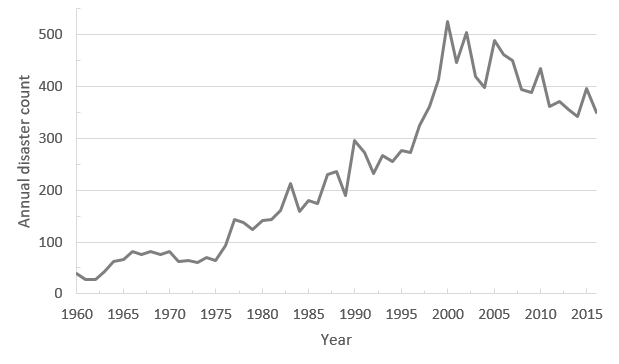
\includegraphics[width=0.9\textwidth]{figs/graph2.png}
	\caption{Natural disaster per year from 1960 to 2016 [From:  EM-DAT: The Emergency Events Database - Universite catholique de Louvain (UCL) - CRED, D. Guha-Sapir - www.emdat.be, Brussels, Belgium]}
	\label{fig:graph1}
\end{figure}

\noindent Around the world, in both wealthy and impoverished regions, individuals and organisations, both governmental and \ac{ngo}, are motivated to reduce and manage the impact of disasters \citep{Coppola2015}. Within this disaster management the decision making process and risk management process are bounded by three key characteristics \citep{Zlatanova2008}. [1.] Rapid action needs to be taken, [2.] aware of the situation and context [3.] with a connected overview of the data available. The goal of the \ac{drm} is to minimize the impact from a disaster \citep{Piero2012}. Information on the extent of the damage is therefore paramount, as demonstrated by relief operations from the \ac{nlrc}. Building damage is an essential indicator for this \citep{Schweier2006}; but can be hard to establish as it requires a lot of manual field labour; an dangerous and timely ordeal for aid workers involved \citep{Kerle2010}. Automated detection of building damages based on remotely sensed data could be the solution, allowing for faster and more efficient response \citep{Vetrivel2016b}. \\

\noindent Remote sensing has long been part of the \ac{drm} cycle. According to \citet{Kerle2015} this started at the beginning of space-based remote sensing around the 1960s and 1970s and brought about the increase in information within the \ac{drm}. From here the development of remote sensing techniques accelerated over the past 50 years and increasingly allows for higher resolution information in a more timely manner. The performance increase in remote sensing solutions make it applicable for the automated classification of building damage \citep{DellAcqua2012,Dong2013}. Many solutions for automated damage detection or classification have been developed over the past years based on several remote sensing techniques. \citet{Dong2013} provides a clear overview of the solutions up until 2013 and several more have been developed since \citep{Dominici2017,Sharma2017,Kakooei2017,Vetrivel2016b,Menderes2015}. However in practice services from the International Charter, like Copernicus and UNOSAT, are mostly used for \ac{sem} \citep{Voigt2016} as they produce usable results \citep{Kerle2010}. The method for damage classification used by these services is manual visual interpretation of remotely sensed data, as is indicated by the disclaimers or map information of products from these services and a program specialist at UNOSAT \citep{Cop2017,UNDAC2017}. While this approach is safer for the aid workers in the field, it remains a laboursome task.


\section{Problem statement}
It is remarkable that the extensive academic research is not implemented in the disaster relief sector, As the building damage is a fundamental indicator used in \ac{drm} and relief operations \citep{Schweier2006}. The lack of implementation of automated methods can be seen as an indicator of the absence of support from the humanitarian agencies. Several considerations could be the cause of this; [1.] there is too little communication between humanitarian agencies and academics, resulting in too complex methods or inadequate solutions. [2.] the methods proposed do not deliver the expected outcomes concerning effectiveness or accuracy. [3.] there are no resources to implement the new methods in existing procedures. An example of this can be found in \citet{Ajmar2011}. This paper mentions the lack of predictable results and time involved as impediments for implementation of automated approaches. Disaster situations require fast implementations as lives might be at stake, while reliable results are necessary for fair distribution of aid. 

This research will establish a method for the accurate classification of building damage after a natural disaster. Existing academic methods will be taken into consideration and tested on the available "real world" data from St. Maarten. Furthermore the research will be conducted in cooperation with \ac{nlrc} to cope with some of considerations that might be causing the lack of implementation. Advances in remote sensing techniques, machine learning and \ac{gis} are recognised as upcoming and supportive technologies within the organisation, as it established a new data team [510] in 2016. The data team and \ac{nlrc}, as well as other humanitarian organisations, could benefit from the research into the automated classification of building damage after a disaster, as it would allow for more efficient delivery of aid and humanitarian relief. The academic field working on remote sensing for disaster situations could also benefit from this research as it will provide a comparison between methods in a scenario different from the academic examples.

\section{Research objectives}


The objective of this research is: \textit{to find a method for the automatic classification of damage inflicted by hurricanes on the island of St. Maarten using remotely sensed data.} Based on the findings of \citet{Kakooei2017} the research will be focused around an implementation from various sources for improvement in the accuracy of the classification To achieve this the following goals have been derived:

\begin{itemize}
	\item Compare existing methods for building damage classification to each other and ground truth data.
	\item Find complementary methods and aspects of data that allow for fusion of data and methods to achieve an increase in accuracy.
	\item Develop a method which fuses the various data sources and methods to facilitate accurate classification of damage to buildings. 
	\item Compare the results from the proposed method to existing methods and ground truth data.
\end{itemize}

With results from these goals the research question will be answered: \textit{Is the fusion of remotely sensed data a viable option for the automatic classification of hurricane inflicted damage?}\\

An viable method would enable humanitarian organisations to accurately plan their interventions and relief operations on the basis of damage inflicted in disaster struck areas. This would allow for an increase in effectiveness of the activities, and therefore help more people affected by a natural disaster. To develop such method various other challenges will need to be handled. These will be dealt with in the literature research and analysis of existing academic methods.\\ 
A description of an effective method is necessary to develop one. To gain insight in the needs and possibilities of methods the following question will need to be answered: Which criteria are most useful for a damage classification framework? With which in turn two other questions are formed, what is damage classification and how does it differ from damage detection? And humanitarian organisations and disaster situations might impose various other criteria on methods. which should therefore be considered in the description as well.\\
The next scientific challenge lies in the determination of the effectiveness of existing methods. The main question to be answered in this regard is the accuracy comparison between ground truth data from St. Maarten and the results from these methods. The fusion of data is expected to improve the accuracy of the various methods, which subsequently will be one of the main indicators within the classification framework. From these results it will be possible to select the aspects of methods and data which will allow for fusion and also result in an accuracy boost in the new method.\\
From the answers to these challenge the new method can be developed but will need to be validated to ensure the results are confirming to expectation and suffice for the use in humanitarian context. To do so the new results will need to be compared to the benchmark results from the existing methods. \\

With answers to all these challenges and the main research question, it would be necessary to see the proposed method on a broader scale and the fit within both the academic field and humanitarian field of operation. This will allow for reflection on the results and might allow for discussion on the possibility of implementation in the field.

\section{research scope}
This research will focus on the accurate and automated classification of building damage in a hurricane struck area. Limitations in a masters thesis are unavoidable as time and resources are limited. Spatially the research is restricted to the Dutch part of the island St. Maarten as well as temporally limited to the aftermath of hurricane Irma in 2017. This limitation is also supported by the fact that the author has been to the island in the aftermath of the hurricanes. This on-the-ground experience could be helpful in the understanding of the problem. \\
The method to be developed will be based on existing methods and will use, for where possible, existing software packages. This will shift the focus from a completely new method, to an adaptation with potential for implementation in various disaster procedures. This allows for more investigation into existing methods, and cherry-picking effective techniques. By choosing approach developing a method which would be added to a list of unused, existing methods, is avoided. To further reduce the scope, only two existing methods will be selected for rigorous assessment. These will be chosen through the theoretical framework and literature research. \\
For this research, the task of object detection, as used by various other academic methods \citep{Vetrivel2016b,Kakooei2017}, will not be used. The datasets available allow for the use of existing building outlines, gathered from recent data. The \ac{nlrc} uses voluntary cartographers to map disaster areas shortly after a disaster and where possible, in case of the hurricane on St. Maarten, shortly before a disaster. Making sure that maps are up to date and can be used for planning. This eliminates the need for object detection from data sources, however requires the data input to be properly matched.\\
The research is limited to the various datasets available through the 510 team of the \ac{nlrc} as cleaning, relief and reconstruction activities on the island make new data collection impossible. However these datasets can be considered a good representation of available data in the wake of large scale disaster. The cooperation with the data team of the \ac{nlrc} allows for a good balance between the technical approach of the Delft University of Technology and a more societal aspect from a humanitarian organisation.\\ 
Section \ref{sec:def} will elaborate some of the scope reductions with literature research.

\section{definition}\label{sec:def}
The International Federation of Red Cross and Red Crescent Societies \citeyearpar{IFRC2017} defines a disaster as follows: 
\begin{quote}
	"A disaster is a sudden, calamitous event that seriously disrupts the functioning of a community or society and causes human, material, and economic or environmental losses that exceed the community’s or society’s ability to cope using its own resources."
\end{quote}
These characteristics in this definition emphasize the need for timely intervention by others outside a community or area to help and support those affected. Ray Shirkhodai notes in \citet[p. i]{AlAchkar2008} that a rapid overview of the situation and extent of damage is necessary to achieve this goal. This is corroborated by \citet{Schweier2006}. To do so with minimum risk to aid workers, the international community established the so-called International Charter \citep{Bessis2003}. With resources from various space agencies around the world it became possible to use \ac{sem} to provide rapid situation awareness after a disaster. However as described by \citet{Kerle2008} there are a diverse selection of other remote sensing techniques which can be used for the collection of data, which could make other forms of \ac{em} possible. This research will take into account this broader approach to remote sensing, looking at advances in \ac{uav} and shrinking data collection technologies as new data sources in the immediate aftermath of a disaster.\\

The implementation of \ac{em} has various scales of resolution. For the purpose of this research these have been categorised as follows:

\begin{itemize}
	\item Damage detection
	\item Damage classification
	\item Damage assessment
\end{itemize}

The lowest resolution considered is damage detection. In this form of \ac{em} the focus is to differentiate between buildings with and without damage. This comparable to the studies that can distinguish between two grades of damage as described by \citet{Dong2013}. An example of this is \citet{Wang2012}, in which image classification is used to derive the difference between buildings damage and not damaged by a disaster.\\

One step up in resolution from detection is the damage classification as used within this research. For classification various grades of damage need to be considered. \cite{Dong2013} describe this as three grades or more. They also provide a framework for five damage classes that can be used in achieving damage classification. These classes are derived from \citet{Grunthal1998}, however the ambiguity introduced with five classes, especially between the three middle grades, is not beneficial for humanitarian aid organisations. Therefore the classification method proposed by \citet{AlAchkar2008} will be used in this research. This framework is focused on damage inflicted to buildings, allows for sufficient variation between damage grades and has example of damage induced by wind. A variation of this is also used by the \ac{nlrc} [available on \href{https://www.510.global/visual-guide-damage-assesment/}{510.global}].\\

The last resolution is damage assessment. This requires more insight in the damage caused, as well as interior damage which is usually not observable in \ac{em} or \ac{sem}. Therefore people on the ground are required to do thorough investigation into the damage caused. The exception to this is the use of high resolution oblique imagery, which in some cases might be able to distinguish damage in the vertical plane \citep{Vetrivel2016a}, however most damage assessment will need to be done by humans with guides from governments, like from \citet{FEMA2016}.\\

\subsection{Hurricane Irma}
One of the major disasters of 2017 was hurricane Irma, being labelled the worst storm in the Caribbean in recorded history \citep{Daniell2017}. In the first week of September this hurricane raged over multiple islands causing billions worth of damage, affecting millions in its path \citep{Phipps2017,Daniell2017}. One of the islands affected is St. Maarten, part of the Kingdom of the Netherlands. It was hit by the eye of the hurricane on the 6th of September with winds up to 185 miles per hour \citep{Wilts2017}. Two other major hurricane passed over the area in the weeks following hurricane Irma, however, fortunately these did little to no extra damage on the island \citep{Gray2017,Bijnsdorp2017}. First damage estimates show that 70 - 90\% of the island may be affected by the storm \citep{Rodekruis2017,UNOSAT2017}. The indication and location of the damage caused is a leading planning tool for organisations like the \ac{nlrc}, providing a first indication of the most vulnerable people in an affected area. Indications of damage have allowed the \ac{nlrc} to help 18.881 individual people since the landfall of hurricane Irma and subsequent relief operation; and long term operations are being started right now to facilitate the rebuilding of the island \citep{Rodekruis2017}. 


